% Options for packages loaded elsewhere
\PassOptionsToPackage{unicode}{hyperref}
\PassOptionsToPackage{hyphens}{url}
%
\documentclass[
]{book}
\usepackage{amsmath,amssymb}
\usepackage{lmodern}
\usepackage{iftex}
\ifPDFTeX
  \usepackage[T1]{fontenc}
  \usepackage[utf8]{inputenc}
  \usepackage{textcomp} % provide euro and other symbols
\else % if luatex or xetex
  \usepackage{unicode-math}
  \defaultfontfeatures{Scale=MatchLowercase}
  \defaultfontfeatures[\rmfamily]{Ligatures=TeX,Scale=1}
\fi
% Use upquote if available, for straight quotes in verbatim environments
\IfFileExists{upquote.sty}{\usepackage{upquote}}{}
\IfFileExists{microtype.sty}{% use microtype if available
  \usepackage[]{microtype}
  \UseMicrotypeSet[protrusion]{basicmath} % disable protrusion for tt fonts
}{}
\makeatletter
\@ifundefined{KOMAClassName}{% if non-KOMA class
  \IfFileExists{parskip.sty}{%
    \usepackage{parskip}
  }{% else
    \setlength{\parindent}{0pt}
    \setlength{\parskip}{6pt plus 2pt minus 1pt}}
}{% if KOMA class
  \KOMAoptions{parskip=half}}
\makeatother
\usepackage{xcolor}
\IfFileExists{xurl.sty}{\usepackage{xurl}}{} % add URL line breaks if available
\IfFileExists{bookmark.sty}{\usepackage{bookmark}}{\usepackage{hyperref}}
\hypersetup{
  pdftitle={1INF03 - Análisis de Datos},
  pdfauthor={Lucio Cornejo},
  hidelinks,
  pdfcreator={LaTeX via pandoc}}
\urlstyle{same} % disable monospaced font for URLs
\usepackage{longtable,booktabs,array}
\usepackage{calc} % for calculating minipage widths
% Correct order of tables after \paragraph or \subparagraph
\usepackage{etoolbox}
\makeatletter
\patchcmd\longtable{\par}{\if@noskipsec\mbox{}\fi\par}{}{}
\makeatother
% Allow footnotes in longtable head/foot
\IfFileExists{footnotehyper.sty}{\usepackage{footnotehyper}}{\usepackage{footnote}}
\makesavenoteenv{longtable}
\usepackage{graphicx}
\makeatletter
\def\maxwidth{\ifdim\Gin@nat@width>\linewidth\linewidth\else\Gin@nat@width\fi}
\def\maxheight{\ifdim\Gin@nat@height>\textheight\textheight\else\Gin@nat@height\fi}
\makeatother
% Scale images if necessary, so that they will not overflow the page
% margins by default, and it is still possible to overwrite the defaults
% using explicit options in \includegraphics[width, height, ...]{}
\setkeys{Gin}{width=\maxwidth,height=\maxheight,keepaspectratio}
% Set default figure placement to htbp
\makeatletter
\def\fps@figure{htbp}
\makeatother
\setlength{\emergencystretch}{3em} % prevent overfull lines
\providecommand{\tightlist}{%
  \setlength{\itemsep}{0pt}\setlength{\parskip}{0pt}}
\setcounter{secnumdepth}{5}
\usepackage{booktabs}
\AtBeginDocument{\renewcommand{\chaptername}{ }}
\ifLuaTeX
  \usepackage{selnolig}  % disable illegal ligatures
\fi
\usepackage[]{natbib}
\bibliographystyle{apalike}

\title{1INF03 - Análisis de Datos}
\author{Lucio Cornejo}
\date{2022-03-25}

\begin{document}
\maketitle

{
\setcounter{tocdepth}{1}
\tableofcontents
}
\hypertarget{about}{%
\chapter*{About}\label{about}}
\addcontentsline{toc}{chapter}{About}

Apuntes del curso \textbf{Análisis de Datos},
dictado en la \emph{Pontificia Universidad Católica del Perú}.

\hypertarget{semana-0321}{%
\chapter{Semana 03/21}\label{semana-0321}}

\hypertarget{viernes}{%
\section{Viernes}\label{viernes}}

\begin{itemize}
\item
  Será necesario hacer un grupo con otros
  estudiantes del curso, con quienes se
  comparta afinidad de investigación, para
  el proyecto final del curso, el cual se
  irá desarrollando a lo largo del curso.
\item
  Python y R son complementatios, no
  es que uno sea \emph{mejor} que el otro.
\item
  Potential project partner:
  \href{C:/Users/HP/Pictures/Screenshots/Captura\%20de\%20pantalla\%20(2118).png}{Screenshot}
\item
  En el curso, usaremos Python en su mayoría,
  pero también se compartirá, después de clase,
  el código análogo ,en R, de lo que trabajemos.
\item
  En la unidades 4 y 5, es donde más podremos
  contrastar el uso de Python y R. De esa manera,
  uno tendría más claro qué lenguaje escoger al
  momento de iniciar algún proyecto particular.
\item
  Fechas de laboratorio\\

  \begin{itemize}
  \tightlist
  \item
    9 abril
  \item
    23 abril
  \item
    7 mayo
  \item
    11 junio
  \item
    25 junio
  \end{itemize}
\item
  \textbf{Las dirigidas (perhaps a veces pcs) se me}
  \textbf{de IOP se me cruzan con todos los labs},
  \textbf{excepto por el primero.}
\end{itemize}

\hypertarget{metodologuxeda-kdd}{%
\subsection{Metodología KDD}\label{metodologuxeda-kdd}}

\hypertarget{quuxe9-es-un-dato}{%
\subsubsection{¿Qué es un dato?}\label{quuxe9-es-un-dato}}

\begin{itemize}
\item
  El dato es el valor de una
  característica/variable/atributo
  (edad, sexo, etc) de la población
  (población delimitada en espacio, tiempo, etc).
\item
  Procesos paralelos
\end{itemize}

Variable
\(\Rightarrow\)
Variable aleatoria
\(\Rightarrow\)
Dato

Población
\(\Rightarrow\)
Muestra
\(\Rightarrow\)
Observación

\begin{itemize}
\tightlist
\item
  La \textbf{información} parte de la unión
  de los datos recopilados.

  \begin{itemize}
  \tightlist
  \item
    Es de utilidad para tomar decisiones.
  \item
    Un solo dato, por su cuenta,
    no nos da información.
  \end{itemize}
\item
  El \textbf{conocimiento} es un conjunto de informaciones
  aplicadas, que permite preveer y planificar.

  \begin{itemize}
  \tightlist
  \item
    La información asociada a un \textbf{contexto} y una
    \textbf{experiencia} se convierte en conocimiento.
  \end{itemize}
\end{itemize}

\hypertarget{descripciuxf3n-de-la-metodologuxeda-kdd}{%
\subsubsection{Descripción de la metodología KDD}\label{descripciuxf3n-de-la-metodologuxeda-kdd}}

\begin{itemize}
\item
  KDD: Knowledge Discovery in Databases
\item
  Algunas definiciones:
\end{itemize}

\begin{quote}
Knowledge Discovery in Databases is
the non trivial process of identifying
valid, novel, potentially useful, and
utimately understandable patterns in data.
\end{quote}

\begin{itemize}
\tightlist
\item
  \emph{Nivel bajo de datos} se refiere a datos que
  no nos dice nada, pero que podría servir para
  generar conocimiento a partir de estos datos.
\end{itemize}

\hypertarget{etapas-de-la-metodologuxeda-kdd}{%
\subsubsection{Etapas de la metodología KDD}\label{etapas-de-la-metodologuxeda-kdd}}

\begin{itemize}
\item
  Esta metodología nos da pasos para cómo
  convertir \textbf{datos} en \textbf{conocimiento}.
\item
  Estas etapas no son obligatorias \ldots{}
  sirven de \textbf{guía}.
\end{itemize}

\begin{figure}

{\centering 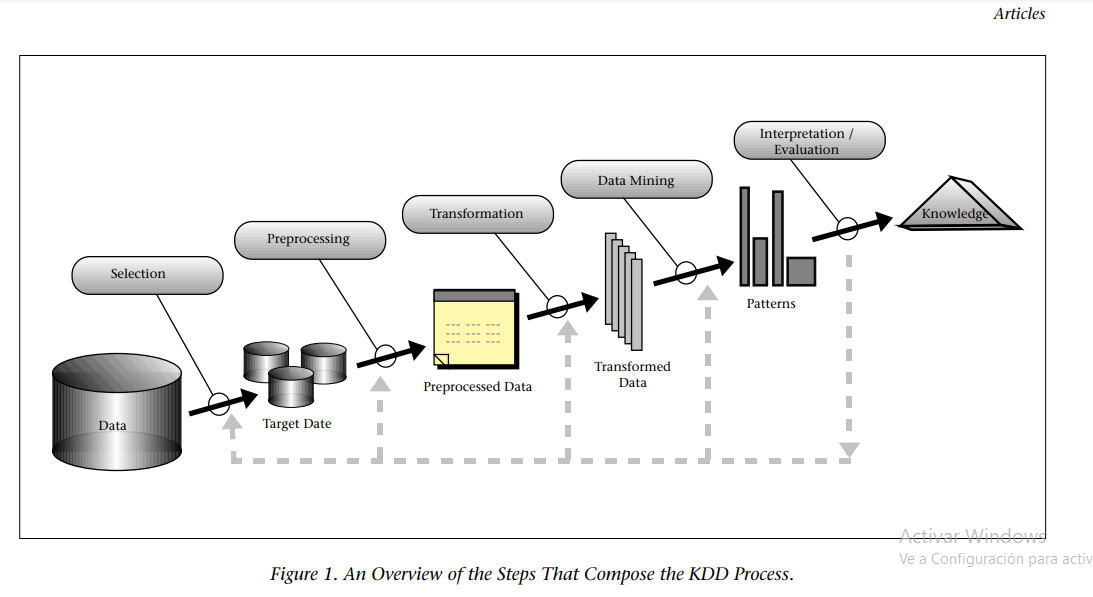
\includegraphics[width=15.18in]{images/etapas-metodologia-kdd} 

}

\caption{Etapas de la metodología KDD}\label{fig:etapas-kdd}
\end{figure}

\begin{itemize}
\item
  En la etapa \textbf{selection}, se reduce la cantidad de data,
  quedándonos con la data que \textbf{nos va a servir} para lograr
  el objetivo de nuestro análisis.\\
  Implica filtrar filas y/o columnas/variables de la data
  (entendida como data frame).\\
  Requiere el entendimiento del objetivo del análisis.
\item
  La parte de información surge en la etapa
  \textbf{Patterns} de la metodología KDD.
  Esa información requiere del bloque
  \emph{interpretation/evaluation} (ver imagen)
  para convertirse en \textbf{knowledge} .
\item
  El paso de \textbf{Transformed data} a
  patterns es vía ``Descriptive methods''.
\end{itemize}

\begin{figure}

{\centering 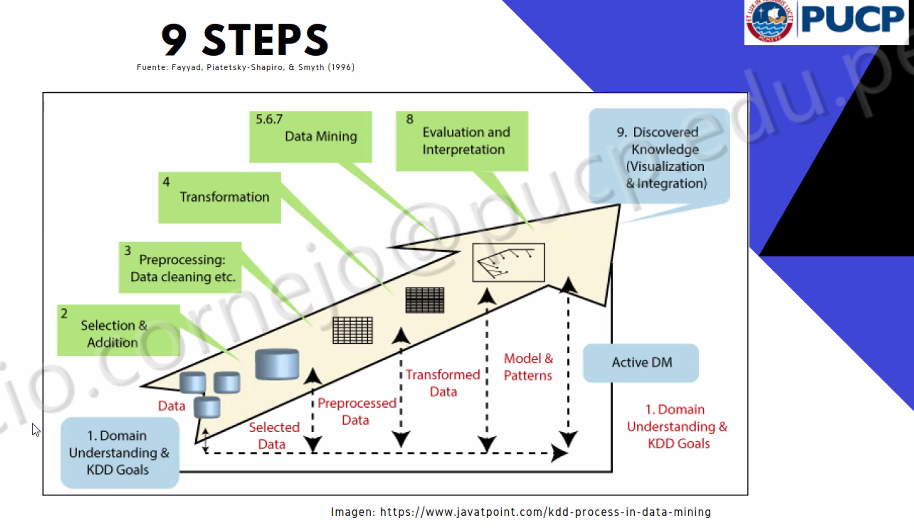
\includegraphics[width=12.69in]{images/etapas-metodologia-kdd-2} 

}

\caption{Etapas (más a detalle) de la metodología KDD}\label{fig:etapas-kdd-2}
\end{figure}

\begin{itemize}
\item
  Las flechas verticales indican que, a medida que avanzamos
  en las etapas, podemos volver al inicio para poder obtener
  nueva data que haya surgido la necesidad de requerir
  para el análisis.
\item
  El bloque \textbf{Active DM (Data Mining)}
  se refiere a que el proceso \emph{Data mining}
  forma parte de TODO el proceso de 9 pasos
  (es otro enfoque).\\
  \textbf{Regresar a cualquier paso es válido}.
\end{itemize}

\begin{enumerate}
\def\labelenumi{\arabic{enumi}.}
\tightlist
\item
  Paso 1

  \begin{itemize}
  \tightlist
  \item
    \textbf{Es el paso principal}.
  \item
    Reunirse con los expertos del tema
    en que se va a trabajar.
    Se discuten cosas como

    \begin{itemize}
    \tightlist
    \item
      ¿Cómo sucede el fenómeno?
    \item
      ¿Qué agentes intervienen con el fenómeno?
    \item
      ¿Qué datos se recolectan
      (variables disponibles) o se pueden recolectar
      para el fenómeno?
    \item
      ¿Para qué población se va a construir
      el proyecto?
    \end{itemize}
  \item
    Se habla en lenguaje entendible
    para todos los expertos, no usando, por
    ejemplo, palabras particulares de Estadística.
  \item
    Se busca \textbf{entender el negocio/problema}.
  \item
    Se busca identificar la \textbf{meta} del proceso
    KDD desde la perspectiva del \textbf{customer}.
  \item
    Es más que nada un proceso \emph{cualitativo}
    que servirá para formalizar el análisis futuro.
  \item
    Es recomendable crear una ficha resumen sobre
    este paso, donde se anota la información
    recopilada en la reunicón (o reuniones) con
    el customer.

    \begin{itemize}
    \tightlist
    \item
      Asignar un experto del negocio como
      encargado del proyecto. Esta persona debe
      ir validando el avance del proyecto, en
      cada uno de los 9 pasos.
    \item
      Anotas una meta principal y las secundarias.
    \item
      Una vez completa esta ficha resumen es
      que podemos pasar al siguiente paso; debe
      redactarse, quedar como evidencia.
    \end{itemize}
  \end{itemize}
\item
  Paso 2

  \begin{itemize}
  \tightlist
  \item
    \textbf{Creating a target data set}.
  \item
    Filtramos la data para obtener un
    subconjunto, tanto en variables (columnas)
    y data samples (filas), al cual se le
    analizará durante pasos siguientes.
  \item
    No se trata de la selección de variable
    que se realiza con código, por ejemplo la
    que busca explicar un fenómeno con las
    variables \emph{independientes}.
  \item
    Esta selección \textbf{no} tiene que ver con
    la \textbf{calidad de datos.} Esa selección
    ocurrirá más adelante.
  \item
    Formalmente, estos filtros se realizan en base a
    \textbf{criterios de inclusión/exclusión}.
  \end{itemize}
\item
  Paso 3

  \begin{itemize}
  \tightlist
  \item
    \textbf{Data cleaning and preprocessing}.
  \item
    Se le dice también \emph{remover el ruido}.
    Donde, el \emph{ruido} hace referencia a los
    \textbf{datos atípicos}.
  \item
    Se ve la forma de trabajar los \emph{datos perdidos}.

    \begin{itemize}
    \tightlist
    \item
      Para construir un modelo, necesitamos lidiar
      primero con los datos perdidos.
    \item
      Dependiendo del contexto, y requiriendo
      fundamento, se pueden imputar/reemplazar los datos
      vacíos por \textbf{cero}, \textbf{la mediana de esa variable},
      etc.
    \item
      Desde el punto de vista de la profesora, máximo
      se debería imputar el 30\% de los valores vacíos de
      una misma variable (que tiene varios valores vacíos).
      Pues, sino, se estaría trabajando con una variable
      \emph{ficticia}, y podría así generar ruido en los
      resultados obtenidos.\\
      Pero eso \textbf{no es una regla}. La decisión de
      imputación dependerá del contexto/fenómeno, y
      debe estar fundamentada \textbf{numéricamente},
      además de tener sentido respecto al negocio.\\
      (Por ejemplo, si imputar una variable por cero
      tiene sentido en cierto contexto particular).
    \end{itemize}
  \item
    Debido, en parte, a estas razones, es importante
    la comunicación constante con un experto del negocio.
  \end{itemize}
\item
  Paso 4

  \begin{itemize}
  \tightlist
  \item
    \textbf{Data reduction and projection}.
  \item
    \textbf{La transformación de la data debe suceder}
    \textbf{después de la limpieza de esta}.
  \end{itemize}
\end{enumerate}

  \bibliography{book.bib,packages.bib}

\end{document}
